\setchapterpreamble[u]{%
    \margintoc\hfil
    \dictum[German Proverb]{Aller Anfang ist schwer.}
}
\chapter{Introduction}
\labch{intro}
% Motivation and preparation for structure

% Paragraphs:

% Context for less familiar readers, broad anchor in space & time
In 1896 the Dutch physicist Pieter Zeemann discovered that the visible spectral lines of a mercury vapour lamp split up in the presence of a magnetic field \sidecite{zeemanInfluenceMagnetismNature1896}. In 1938 Isidor Rabi then first described nuclear \acrfull{mr} \sidecite{rabiNewMethodMeasuring1938}. His technique was in turn extended by Felix Bloch \sidecite{blochNuclearInductionExperiment1946} and Edward Mills Purcell \sidecite{purcellResonanceAbsorptionNuclear1946} and is nowadays one of the most powerful tools in analytical sciences. It can be used for analysing the structure of molecular systems, studying crystals and imaging in medicine among others. In 1966 Richard Robert Ernst developed \acrfull{ftnmr} \sidecite{ernstApplicationFourierTransform1966}, which is the same fundamental technique still used today.

% Need for the work, i.e. what the scientific community has vs what they want
Since then, the technology has advanced fast to higher magnetic field strengths and higher processing power. Enabling better images, higher resolutions and new technology magnetic resonance has become an essential part of many scientists' toolboxes. Unfortunately, higher capabilities come hand in hand with higher costs.

Not much effort has gone towards using the technological advancements of recent decades to lower the cost of magnetic resonance technology. Therefore, there are myriads of lost opportunities in education, industry and research. The global south is disproportionally affected by this trend. This can be seen easily when looking at the number of NMR publications published in a given country in \reffig{nmr_citations}. This is in line with the growing disparity in citations \sidecite{nielsenGlobalCitationInequality2021}.
\begin{figure}[h!bt]
    \centering
    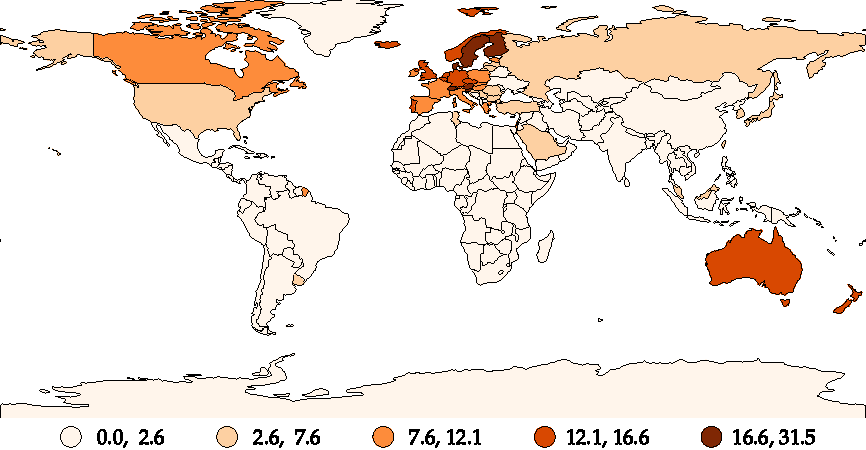
\includegraphics{data/nmr_citations/nmr-affiliations-per-million-people_naturalbreaks.pdf}
    \caption{\captiontitle{\enquote{NMR publications} per million capita (2021)}. Countries coloured in white have no access to NMR, while Switzerland appears as a global leader in NMR science. (Dr. Maria Pechlaner, Infozentrum Chem. Biol. Pharm., ETH Zürich; database: Scopus)}
    \labfig{nmr_citations}
\end{figure}

NMR is used across various fields, making the lack of NMR specialists in the Global South a dire problem. It is used in research --- as an example --- for chemical, physical and structural analysis and drug discovery. It is used in medicine for non-invasive imaging with the famous \acrshort{mri} machine, in industry for process control in the petroleum industry or drug screening and in education to teach concepts of NMR, quantum mechanics and even fundamentals of quantum computing. The lack of NMR technology thus affects a broad range of fields.

% Indicate what I have done (i.e. the task)
To tackle this problem, the presented work focuses on lowering the entry barrier to magnetic resonance research, specifically \acrfull{nmr}. Consequently, we developed a low-cost easy-to-use easy-to-build low-field \acrshort{nmr} spectrometer. The detailed, hands-on documentation includes specifications, simulations, full hardware descriptions, CAD designs Python control code and reproducible measurement results\sidenote{The full documentation including the source codes is currently available at the \href{https://gitlab.ethz.ch/mstabel/nmr-spectrometer}{official ETH Zürich Gitlab} (\url{https://gitlab.ethz.ch/mstabel/nmr-spectrometer})}.

% Preview of the paper to prepare for structure
First, the general concept of an \acrshort{nmr} spectrometer is briefly introduced in \refch{concepts}, which is then expanded upon in detail when describing the individual parts of the built spectrometer in \refch{methods}. Details on the building process and lessons learned for the interested reader can be found in \refch{building-process} and \refch{lessons-learned}. Having delved into all the parts of an \acrshort{nmr} spectrometer \refch{results} presents the measurement results obtained with the built spectrometer. Finally, \refch{conclusion} presents the conclusion and high-level achievements of this work together with an outlook of still-to-be-done tasks.
